% !TEX root = ../TensorOT.tex

%%%%%%%%%%%%%%%%%%%%%%%%%%%%%%%%%%%%%%%%%%%%%%%%%%%%%%%%%
\section{Quantum Sinkhorn}
\label{eq-q-sink}

The convex program~\eqref{eq-Kantorovich} defining quantum OT is computationally challenging because it can be very large scale (problem size is $|I| \times |J|$) for imaging applications, and it involves matrix exponential and logarithm. In this section, leveraging recent advances in computational OT initiated by Cuturi~\shortcite{cuturi-2013}, we propose to use a similar entropy regularized strategy (see also section~\ref{sec-intro}), but this time with the quantum entropy~\eqref{eq-h-quantum}. 

%%%%%%%%%%%%%%%%%%%%%%%%%%%%%%%%%%%%%%%%%%%%%%%%%%%%%%%%%
\subsection{Entropic Regularization}

We define an entropic regularized version of~\eqref{eq-Kantorovich}
\eql{\label{eq-Kantorovich-regul}
	W_\epsilon(\mu,\nu) \eqdef \min_{\ga} \dotp{\ga}{c} + \rho_1\KL(\ga \ones_J|\mu) + \rho_2\KL(\ga^\top \ones_I|\nu) - \epsilon H(\ga). 
}
Note that when $\epsilon=0$, one recovers the original problem~\eqref{eq-Kantorovich}. 
%
This is a strongly convex program, with a unique solution. The crux of this approach, as already known in the scalar case (see~\cite{2016-chizat-sinkhorn}), is that its convex dual has a particularly simple structure, which is amenable to a simple alternating maximization strategy. 

\begin{prop}
	The dual problem associated to~\eqref{eq-Kantorovich-regul} reads
	\begin{multline}\label{eq-dual-pb}
		W_\epsilon(\mu,\nu)
		= 
		\umax{u,v} -\!
				\tr\Big[
						\rho_1 \sum_i (e^{u_i+\log(\mu_i)} - \mu_i) \\
					+   \rho_2 \sum_j (e^{v_j+\log(\nu_j)} - \nu_j)
					+    \epsilon \sum_{i,j}  e^{ \Kern(u,v)_{i,j} }
			 \Big], 
	\end{multline}	
	where $u=(u_i)_{i \in I}, v=(v_j)_{j \in J}$ are collections of arbitrary symmetric (not necessarily in $\Ss_+^d$) matrices $u_i, v_j \in \Ss^d$, 
	where we define
	\eql{\label{eq-defn-K}
		\Kern(u,v)_{i,j} \eqdef -\frac{c_{i,j} + \rho_1 u_i + \rho_2 v_j}{\epsilon}.
	} 
	% where we use the notation $u \ones^\top + \ones v^\top \eqdef (u_i+v_j)_{i,j}$. 
	Furthermore, the following primal-dual relationships hold at optimality:
	\eql{\label{eq-primal-dual-scaling}
		\foralls (i,j), \quad \ga_{i,j} = \exp\pa{ \Kern(u,v)_{i,j} }.
	}
\end{prop}
\begin{proof} \if 0
Applying the Fenchel--Rockafellar duality theorem \justin{cite me!} to~\eqref{eq-Kantorovich-regul} leads to the dual program
\eq{
	\umax{u,v} - \epsilon H^*( \Kern(u,v) |\xi) 
	-\rho_1 \KL^*(u|\mu) - \rho_2 \KL^*(v|\nu) - \epsilon \tr(\xi), 
}
where here $\KL^*(\cdot|\mu)$ corresponds to the Legendre transform with respect to the first argument of the KL divergence.
%
The following Lengendre--Fenchel \justin{cite me!} formula leads to the desired result:
%\eq{
%	(-H)^*(u) = \tr( \exp(u) ), 
%}
\begin{align*} % eq-legendre-kl
	H^*(K) &= \textstyle\sum_{i,j} \tr( e^{K_{i,j}} ) \\
	\KL^*(u|\mu) &= \textstyle\sum_i \tr( \exp(u_i+\log(\mu_i)) - \mu_i).
\end{align*}
%
\lenaic{replace w/ the following proof (after double check):}
\fi
Applying the Fenchel--Rockafellar duality theorem~\cite{rockafellar-convex} to~\eqref{eq-Kantorovich-regul} leads to the dual program
\eq{
	\umax{u,v} - \epsilon \KL^*( \Kern_0(u,v)|\xi) 
	-\rho_1 \KL^*(u|\mu) - \rho_2 \KL^*(v|\nu) - \epsilon \tr(\xi), 
}
where here $\KL^*(\cdot|\mu)$ corresponds to the Legendre transform with respect to the first argument of the KL divergence, $ \Kern_0(u,v)_{i,j} \eqdef -\frac{\rho_1 u_i + \rho_2 v_j}{\epsilon}$ and $\xi_{i,j} \eqdef \exp(-c_{i,j}/\epsilon)$ for all $i,j$.
%
The following Lengendre formula leads to the desired result:
%\eq{
%	(-H)^*(u) = \tr( \exp(u) ), 
%}
\eq{% eq-legendre-kl
	\KL^*(u|\mu) = \textstyle\sum_i \tr( \exp(u_i+\log(\mu_i)) - \mu_i).
}
\end{proof}


%%%%%%%%%%%%%%%%%%%%%%%%%%%%%%%%%%%%%%%%%%%%%%%%%%%%%%%%%
\subsection{Quantum Sinkhorn Algorithm}

It is possible to use Dykstra's algorithm~\shortcite{Dykstra83} (see~\cite{bauschke-lewis} for its extension to Bregman divergences) to solve~\eqref{eq-dual-pb}. This corresponds to alternatively maximizing~\eqref{eq-dual-pb} with respect to $u$ and $v$. 
%
The following proposition states that the maximization with respect to either $u$ or $v$ leads to two fixed-point equations. 
%
These fixed points are conveniently written using the log-sum-exp operator, 
\eql{\label{eq-dfn-lse}
	\LSE_j( K ) \eqdef \Big( \log \sum_j \exp(K_{i,j}) \Big)_i, 
}
where the sum on $j$ is replaced by a sum on $i$ for $\LSE_i$. 

\begin{prop}\label{prop-fixed-points}
	For $v$ fixed (resp.\ $u$ fixed), the minimizer $u$ (resp.\ $v$) of~\eqref{eq-dual-pb} satisfies
	\begin{align}\label{eq-fixed-point-u}
		\foralls i, \quad u_i = \LSE_j(\Kern(u,v))_i-\log(\mu_i), \\
		\foralls j, \quad v_j = \LSE_i(\Kern(u,v))_j-\log(\nu_j), \label{eq-fixed-point-v}
	\end{align}
	where $\Kern(u,v)$ is defined in~\eqref{eq-defn-K}.
\end{prop}
\begin{proof}
	Writing the first order condition of~\eqref{eq-dual-pb} with respect to each $u_i$ leads to
	\eq{
		\rho_1 e^{u_i + \log(\mu_i)} - \rho_1 \sum_{j} e^{\Kern(u,v)_{i,j}} = 0
	} 
	which gives the desired expression. A similar expression holds for the first order conditions with respect to $v_j$.
\end{proof}

A simple fixed point algorithm is then obtained by replacing the explicit alternating minimization with respect to $u$ and $v$ in Dykstra's with just one step of fixed point iteration~\eqref{eq-fixed-point-u} and~\eqref{eq-fixed-point-v}. To make the resulting fixed point contractant and ensure linear convergence, one introduces relaxation parameters $(\tau_1,\tau_2)$. 

The quantum Sinkhorn algorithm is detailed in Algorithm~\ref{alg:sinkhorn}. It alternates between the updates of $u$ and $v$, using relaxed fixed point iterations associated to~\eqref{eq-fixed-point-u} and~\eqref{eq-fixed-point-v}. We use the following $\tau$-relaxed assignment notation 
\eql{\label{eq-dfn-relaxed-assign}
	a \RelaxAssign{\tau} b 
	\quad\text{means that}\quad
	a \leftarrow (1-\tau) a + \tau b.
}
The algorithm outputs the scaled kernel $\ga_{i,j} = \exp(K_{i,j})$.


\begin{rem}[Choice of $\tau_k$]\label{rem-choice-tau}
 In the scalar case, i.e. $d=1$ (and also for isotropic input tensors), when using $\tau_k = \tfrac{\epsilon}{\rho_k+\epsilon}$ for $k=1,2$, one retrieves exactly Sinkhorn iterations for unbalanced transport as described in~\cite{2016-chizat-sinkhorn}, and each update of $u$ (resp.\ $v$) exactly solves the fixed point~\eqref{eq-fixed-point-u} (resp.\ \eqref{eq-fixed-point-v}). 
%
Moreover, it is simple to check that these iterates are contractant whenever
\eq{
	\tau_k \in ]0,\tfrac{2 \epsilon}{\epsilon+\rho_k}[
	\quad\text{for } k=1,2.
}
	and this property has been observed experimentally for higher dimensions $d=2,3$. Using higher values for $\tau_k$ actually often improves the (linear) convergence rate. Figure~\ref{fig:speed} displays a typical example of convergence, and exemplifies the usefulness of using large values of $\tau_k$, which leads to a speed-up of a factor 6 with respect to the usual Sinkhorn's choice $\tau_k=\tfrac{\epsilon}{\epsilon+\rho_k}$.
\end{rem}

%%% FIG %%%
\begin{figure}\centering
\begin{tabular}{@{}c@{\hspace{1mm}}c@{}}
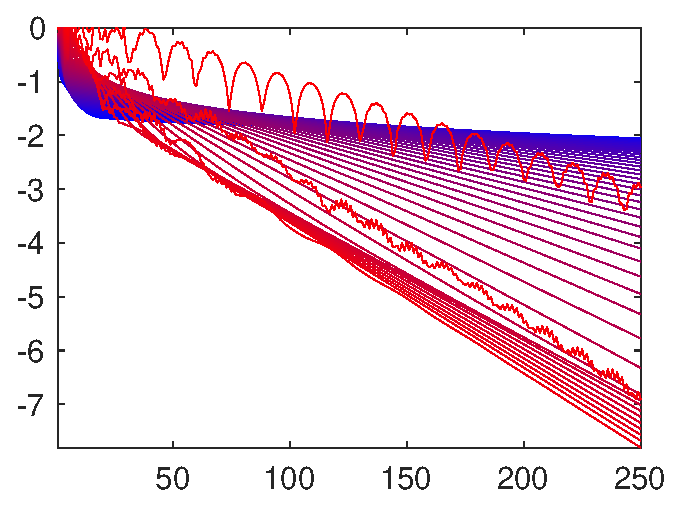
\includegraphics[width=.49\linewidth]{speed/convergence-curve}&
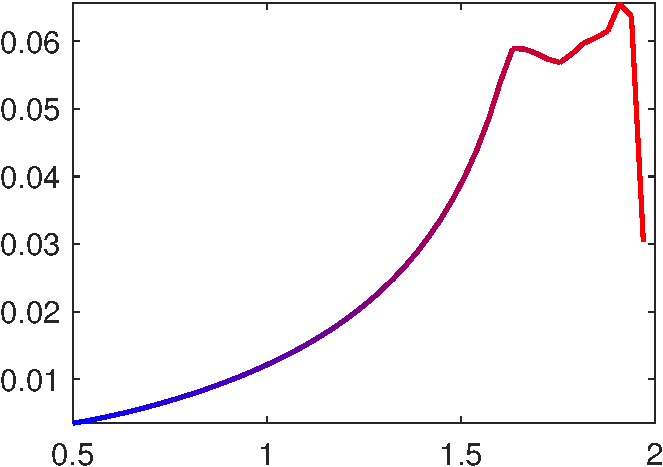
\includegraphics[width=.49\linewidth]{speed/convergence-rate}\\
$\log_{10}\norm{v^{(t+1)}-v^{(t)}}_\infty$ vs $t$ & 
Rate $\kappa$ vs. $\al$
\end{tabular}
\caption{Display of convergence of Sinkhorn Algorithm~\ref{alg:sinkhorn} for the example displayed on the first row of Figure~\ref{fig:intro}. 
%
Denoting $v^{(t)}$ the value of the variable $v$ at iteration $t$, the left plot shows the fixed point residual error for increasing values of $\tau_1=\tau_2=\tfrac{\al\epsilon}{\epsilon+\rho}$ with $\al \in [0.5,2]$ (blue to red). 
%
The algorithm exhibits a linear convergence rate, $\log_{10}\norm{v^{(t+1)}-v^{(t)}}_\infty \sim - \kappa t$ for some $\kappa>0$, and the right plot displays $\kappa$ as a function of $\al$.  
} \label{fig:speed}
\end{figure}
%%% FIG %%%


\begin{rem}[Stability]In contrast to the usual implementation of Sinkhorn's algorithm, which is numerically unstable for small $\epsilon$ because it requires to compute $e^{u/\epsilon}$ and $e^{v/\epsilon}$, the proposed iterations using the LSE operator are stable. The algorithm can thus be run for arbitrary small $\epsilon$, although the linear speed of convergence is of course impacted.   
\end{rem}

\begin{algorithm}[t]
\fbox{\hspace{-.1in}\parbox{\columnwidth}{%
\begin{algorithmic}
\Function{Quantum-Sinkhorn}{$\mu,\nu,c,\epsilon,\rho_1,\rho_2$}
	\algspace
	\State $\foralls k=1,2, \quad \tau_k \in ]0,\tfrac{2 \epsilon}{\epsilon+\rho_k}[$, 
	\Let{$\foralls (i,j) \in I \times J, \quad (u_i,v_j)$}{$(0_{d \times d}, 0_{d \times d})$}
	\For{$s=1,2,3,\ldots$}
		\Let{$K$}{$\Kern(u,v)$}
		\State $\foralls i \in I, \quad u_i \RelaxAssign{\tau_1} \LSE_j(K_{i,j})-\log(\mu_i)$
		\Let{$K$}{$\Kern(u,v)$}
		\State $\foralls j \in J, \quad v_j \RelaxAssign{\tau_2} \LSE_i(K_{i,j})-\log(\nu_j)$
	\EndFor
	\State\Return{$(\ga_{i,j} = \exp(K_{i,j}))_{i,j}$}
\EndFunction
  \end{algorithmic}
}}
\caption{Quantum-Sinkhorn iterations to compute the optimal coupling $\ga$ of the regularized transportation problem~\eqref{eq-Kantorovich-regul}. The operator $\Kern$ is defined in~\eqref{eq-defn-K}.\label{alg:sinkhorn}}
\end{algorithm}

\begin{rem}[log and exp computations]
A major computational workload of the Q-Sinkhorn Algorithm~\ref{alg:sinkhorn} is the repetitive computation of matrix exp and log. 
%
For $d \in \{2,3\}$ it is possible to use closed-form expressions to diagonalize the tensors, so that the overall complexity is comparable with the usual scalar case $d=1$.
%
While the applications in Section~\ref{sec:appli} only require these low-dimensional settings, high dimensional problems are of interest, typically for machine learning applications.  In these cases, one has to resort to iterative procedures, such as rapidly converging squaring schemes~\cite{HighamExp,HighamLog}.
\end{rem}

\begin{rem}[Computational complexity]
For low-dimensional problems (typically for those considered in Section~\ref{sec:appli}), the Q-Sinkhorn Algorithm~\ref{alg:sinkhorn} scales to grid sizes of roughly 5k points (with machine-precision solutions computed in a few minutes on a standard laptop).
%
For large scale grids, even storing the full coupling $\ga$ becomes prohibitive. We however observed numerically that, similarly  to the usual scalar case, the optimal $\ga$ solving~\eqref{eq-Kantorovich-regul} is highly sparse (up to machine precision for small enough $\epsilon$).
% 
We thus found that the use of the multi-scale refinement strategy introduced in~\cite{Schmitzer2016} is able to make the Q-Sinkhorn scale to high resolution grids.  It is not used to produce the figures of this article, but it is available in the companion computational toolbox.
\end{rem}

\begin{rem}[Gurvits' non-commutative Sinkhorn]
Let us insist on the fact that the proposed Q-Sinkhorn Algorithm~\ref{alg:sinkhorn} is unrelated to Gurvits' Sinkhorn algorithm~\cite{gurvits2004classical}. While Gurvits' iterations compute a coupling between a pair of input tensors, our method rather couples two \textit{fields} of tensors (viewed as tensor-valued measures). Our usage of the wording  ``quantum'' refers to the notion of quantum entropy~\eqref{eq-h-quantum} and is not inspired by quantum physics.
\end{rem}


%%%%%%%%%%%%%%%%%%%%%%%%%%%%%%%%%%%%%%%%
\subsection{Trace-Constrained Extension}

The quantum OT problem~\eqref{eq-Kantorovich} does not impose that the marginals of the coupling $\gamma$ match exactly the inputs $(\mu,\nu)$. It is only in the limit $(\rho_1,\rho_2) \rightarrow (+\infty,+\infty)$ that an exact match is obtained, but as explained in Section~\ref{sec-tensor-ot}, this might leads to an empty constraint set.

To address this potential issue, we propose to rather only impose the \textit{trace} of the marginals to match the trace of the input measures, in order to guarantee conservation of mass (as measured by the trace of the tensors). We thus propose to solve the entropy regularized problem~\eqref{eq-Kantorovich-regul} with the extra constraint
\eq{
	\foralls i \in I, \quad \sum_j \tr(\ga_{i,j}) = \tr(\mu_i) \qandq
	\foralls j \in J, \quad \sum_i \tr(\ga_{i,j}) = \tr(\nu_j).
}
These two extra constraints introduce two dual Lagrange multipliers $(\al,\be) \in \RR^I \times \RR^J$ and the optimal coupling relation~\eqref{eq-primal-dual-scaling} is replaced by 
\eq{\label{eq-primal-dual-scaling_bis}
		\foralls (i,j), \quad \ga_{i,j} = \exp\pa{ \Kern(u,v,\al,\be)_{i,j} }
}
\eq{
		\qwhereq
		\Kern(u,v,\al,\be)_{i,j} \eqdef -\frac{c_{i,j} + \rho_1 u_i + \rho_2 v_j + \al_i + \be_j}{\epsilon}.
}

Q-Sinkhorn algorithm~\ref{alg:sinkhorn} is extended to handle these two extra variables $(\al,\be)$ by simply adding two steps to update these variables
\begin{align*}
	\foralls i \in I, \quad \al_i \leftarrow \al_i + \epsilon \LSTE_j( K )_i \qwhereq K \eqdef \Kern(u,v,\al,\be), \\
	\foralls j \in J, \quad \be_j \leftarrow \be_j + \epsilon \LSTE_i( K )_j \qwhereq K \eqdef \Kern(u,v,\al,\be).
\end{align*}
where we introduced the log-sum-trace-exp operator
\eq{
	\LSTE_j( K ) \eqdef \Big( \log \sum_j \tr( \exp(K_{i,j}) ) \Big)_i
}
(and similarly for $\LSTE_i$). Note that in this expression, the $\exp$ is matrix-valued, whereas the $\log$ is real-valued.


%%%%%%%%%%%%%%%%%%%%%%%%%%%%%%%%%%%%%%%%
\subsection{Numerical Illustrations}
\label{sec-numerics-interp}

Figures~\ref{fig:intro},~\ref{fig:1d-interp} and~\ref{fig:qot-vs-ot} illustrate on synthetic examples of input tensor fields $(\muA,\muB)$ the Q-OT interpolation method. 
%
We recall that it is obtained in two steps:
\begin{enumerate}
	\item One first computes the optimal $\ga$ solving~\eqref{eq-Kantorovich-regul} using Sinkhorn iterations (Algorithm~\ref{alg:sinkhorn}).
	\item Then, for any $t \in [0,1]$, one computes $\mu_t$ using this optimal $\ga$ with formula~\eqref{eq-interpolating}.
\end{enumerate}
   
Figure~\ref{fig:1d-interp} shows examples of interpolations on a 1-D domain $X=Y=[0,1]$ with tensors of dimension $d=2$ and $d=3$, and a ground cost $c_{i,j}=|x_i-y_j|^2\Id_{d \times d}$. It compares the OT interpolation, which achieves a ``mass displacement,'' to the usual linear interpolation $(1-t)\mu+t\nu$, which only performs a pointwise interpolation of the tensors. 

Figure~\ref{fig:qot-vs-ot} shows the effect of taking into account the anisotropy of tensors into the definition of OT. In the case of isotropic tensors (see Remark~\ref{rem-classical-ot}), the method reduces to the usual scalar OT, and in 1-D it corresponds to the monotone re-arrangement~\cite{santambrogio2015optimal}. In contrast, the Q-OT of anisotropic tensors is forced to reverse the ordering of the transport map in order for tensors with similar orientations to be matched together. 
%
This example illustrates that the behaviour of our tensor interpolation is radically different from only applying classical scalar-valued OT to the trace of the tensor (which would result in the same coupling as the one obtained with isotropic tensors, Figure~\ref{fig:qot-vs-ot}, left). 

Figure~\ref{fig:intro} shows larger scale examples. 
%
The first row corresponds to $X=Y=[0,1]^2$ and $d=2$, with cost $c_{i,j}=\norm{x_i-y_j}^2\Id_{2 \times 2}$, which is a typical setup for image processing.
%
The second row corresponds to $X=Y$ being a triangulated mesh of a surface, and the cost is proportional to the squared geodesic distance $c_{i,j}=d_X(x_i,y_j)^2 \Id_{2\times 2}$. 

% !TEX root = ../TensorOT.tex

%%% FIG %%%
\begin{figure}\centering
\begin{tabular}{@{}c@{}|@{}c@{}}
\includegraphics[width=.49\linewidth]{1d/cross-orient/linear-interp}&
\includegraphics[width=.49\linewidth]{1d/cross-orient/interp-ellipses}\\\hline
\includegraphics[width=.49\linewidth]{3d/plate-elong/linear-interp}&
\includegraphics[width=.49\linewidth]{3d/plate-elong/interp-ellipses}\\\hline
Linear interpolation & Quantum OT
\end{tabular}
\caption{Comparison of linear and quantum-OT interpolation (using formula~\eqref{eq-interpolating}). 
Each row shows a tensor field $\mu_t$ (top $d=2$, bottom $d=3$) along a linear segment from $t=0$ to $t=1$ ($t$ axis is vertical).
} \label{fig:1d-interp}
\end{figure}
%%% FIG %%%

%%% FIG %%%
\begin{figure}\centering
\begin{tabular}{@{}c@{}|@{}c@{}}
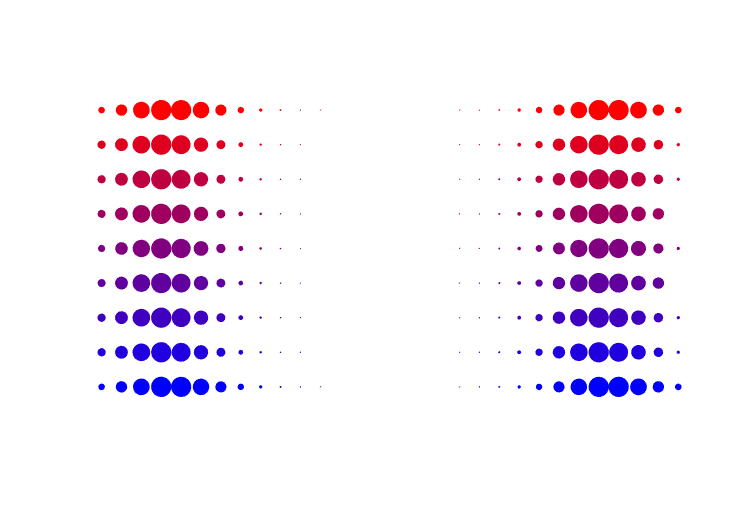
\includegraphics[width=.49\linewidth,trim=40 55 30 48,clip]{1d/dirac-pairs/interp-ot}&
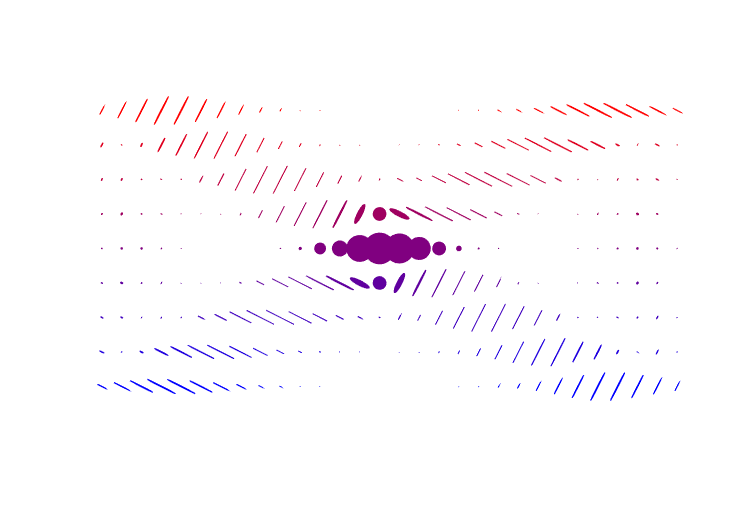
\includegraphics[width=.49\linewidth,trim=40 55 30 48,clip]{1d/dirac-pairs/interp-qot}\\\hline
Classical OT & Quantum OT
\end{tabular}
\caption{Comparison of classical OT (i.e. between isotropic tensors) and quantum-OT (between anisotropic tensors) interpolation (using formula~\eqref{eq-interpolating}), using the same display as Figure~\ref{fig:1d-interp}. 
} \label{fig:qot-vs-ot}
\end{figure}
%%% FIG %%%
